\documentclass[12pt]{book}

\newcommand{\thetitle}{Think Java: How to Think Like a Computer Scientist}
\title{\thetitle}

\newcommand{\theauthors}{Allen Downey and Chris Mayfield}
\author{\theauthors}

\newcommand{\theversion}{Version 6.0 Draft -- \today}
\date{\theversion}

\usepackage{geometry}
\geometry{
    width=5.5in,
    height=8.5in,
    hmarginratio=3:2,
    vmarginratio=1:1,
    includehead=true,
    headheight=15pt
}

% paragraph spacing
\setlength{\parindent}{0pt}                      % 17.62482pt
\setlength{\parskip}{12pt plus 4pt minus 4pt}    % 0.0pt plus 1.0pt
\linespread{1.05}
\def\arraystretch{1.5}

% list spacing
\setlength{\topsep}{5pt plus 2pt minus 3pt}      % 10.0pt plus 4.0pt minus 6.0pt
\setlength{\partopsep}{-6pt plus 2pt minus 2pt}  %  3.0pt plus 2.0pt minus 2.0pt
\setlength{\itemsep}{0pt}                        %  5.0pt plus 2.5pt minus 1.0pt

% these are copied from tex/latex/base/book.cls
% all I changed is afterskip
\makeatletter
\renewcommand{\section}{\@startsection {section}{1}{\z@}%
    {-3.5ex \@plus -1ex \@minus -.2ex}%
    {0.7ex \@plus.2ex}%
    {\normalfont\Large\bfseries}}
\renewcommand\subsection{\@startsection{subsection}{2}{\z@}%
    {-3.25ex\@plus -1ex \@minus -.2ex}%
    {0.3ex \@plus .2ex}%
    {\normalfont\large\bfseries}}
\renewcommand\subsubsection{\@startsection{subsubsection}{3}{\z@}%
    {-3.25ex\@plus -1ex \@minus -.2ex}%
    {0.3ex \@plus .2ex}%
    {\normalfont\normalsize\bfseries}}
\makeatother

% table of contents vertical spacing
\usepackage{tocloft}
\setlength\cftparskip{8pt plus 4pt minus 4pt}

% The following line adds a little extra space to the column
% in which the Section numbers appear in the table of contents
\makeatletter
\renewcommand{\l@section}{\@dottedtocline{1}{1.5em}{3.0em}}
\makeatother

% customize page headers
\usepackage{fancyhdr}
\pagestyle{fancyplain}
\renewcommand{\chaptermark}[1]{\markboth{Chapter \thechapter ~~ #1}{}}
\renewcommand{\sectionmark}[1]{\markright{\thesection ~~ #1}}
\lhead[\fancyplain{}{\bfseries\thepage}]%
      {\fancyplain{}{\bfseries\rightmark}}
\rhead[\fancyplain{}{\bfseries\leftmark}]%
      {\fancyplain{}{\bfseries\thepage}}
\cfoot{}
%\rfoot{\textcolor{gray}{\tiny ThinkJava Draft \today}}

% balanced index with TOC entry
\usepackage{makeidx}
\makeindex
%\usepackage[totoc]{idxlayout}

% automatically index glossary terms
\newcommand{\term}[1]{%
\index{#1}
\item[#1:]}
% TODO: doesn't work with plastex
%\newcommand{\term}[1]{\item[#1:]}

% where to find graphics
\usepackage{graphicx}
%\graphicspath{{figs/}}

%% tweak spacing of figures and captions
%\usepackage{floatrow}
%\usepackage{caption}
%\captionsetup{
%    font=small,
%    labelformat=empty,
%    justification=centering,
%    skip=4pt
%}

% format end of chapter excercises
\usepackage{amsmath}
\usepackage{amsthm}
\newtheoremstyle{exercise}
  {12pt}        % space above
  {12pt}        % space below
  {}            % body font
  {}            % indent amount
  {\bfseries}   % head font
  {}            % punctuation
  {12pt}        % head space
  {}            % custom head
\theoremstyle{exercise}
\newtheorem{exercise}{Exercise}[chapter]

% colors for code listings and output
\usepackage{xcolor}
\definecolor{bgcolor}{HTML}{FAFAFA}
\definecolor{comment}{HTML}{007C00}
\definecolor{keyword}{HTML}{0000FF}
\definecolor{strings}{HTML}{B20000}

% syntax highlighting in code listings
\usepackage{textcomp}
\usepackage{listings}
\lstset{
    language=java,
    basicstyle=\ttfamily,
    backgroundcolor=\color{bgcolor},
    commentstyle=\color{comment},
    keywordstyle=\color{keyword},
    stringstyle=\color{strings},
    columns=fullflexible,
    keepspaces=true,
    showstringspaces=false,
    upquote=true,
    aboveskip=\parskip,
    belowskip=\parskip
}

% code listing environments
\lstnewenvironment{code}
{\minipage{\linewidth}}
{\endminipage}
\lstnewenvironment{stdout}
{\lstset{commentstyle=,keywordstyle=,stringstyle=}\minipage{\linewidth}}
{\endminipage}

% pdf hyperlinks, table of contents, and document properties
\usepackage[pdftex]{hyperref}
\hypersetup{%
  pdftitle={\thetitle},
  pdfauthor={\theauthors},
  pdfsubject={\theversion},
  pdfkeywords={},
  bookmarksopen=false,
  colorlinks=true,
  citecolor=black,
  filecolor=black,
  linkcolor=black,
  urlcolor=blue
}

% inline syntax formatting
\newcommand{\java}[1]{\lstinline{#1}} %\end{
%\newcommand{\java}[1]{\verb"#1"}
%\newcommand{\java}[1]{{\tt #1}}

\begin{document}
\setcounter{chapter}{13}


\chapter{Object-oriented programming}

If you haven't done the exercises in Chapters~\ref{gridworld} and
\ref{gridworld2}, you should do them before reading this chapter.
As a reminder, you can find the
documentation for the GridWorld classes at
\url{http://www.greenteapress.com/thinkapjava/javadoc/gridworld/}.

Part 3 of the GridWorld Student Manual presents the classes that
make up GridWorld and the interactions among them.  It is an
example of object-oriented design and an opportunity to discuss OO
design issues.

But before you read the Student Manual, there are a few more things
you need to know.


\section{Programming paradigms}

\index{programming language}
\index{language!programming}
\index{programming style}
\index{object-oriented programming}
\index{functional programming}
\index{procedural programming}
\index{programming!object-oriented}
\index{programming!functional}
\index{programming!procedural}

There are many programming languages and almost as many
programming styles (sometimes called paradigms).
The programs we have written so far are {\bf procedural},
because the emphasis has been on specifying computational procedures.

Most Java programs are {\bf object-oriented}, which means that
the focus is on objects and their interactions.
Here are some of the characteristics of object-oriented programming:

\begin{itemize}

\item Objects often represent entities in the real world.
  In the previous chapter, creating the {\tt Deck} class
  was a step toward object-oriented programming.

\item The majority of methods are object methods (like the methods you
  invoke on {\tt Strings}) rather than class methods (like the {\tt Math}
  methods).  The methods we have written so far have
  been class methods.  In this chapter we write some object methods.

\item Objects are isolated from each other by limiting the ways they
  interact, especially by preventing them from accessing
  instance variables without invoking methods.

\item Classes are organized in family trees where
  new classes extend existing classes, adding new methods and
  replacing others.

\end{itemize}

In this chapter I translate the {\tt Card} program from the
previous chapter from procedural to object-oriented style.  You
can download the code from this chapter from
\url{http://thinkapjava.com/code/Card3.java}.


\section{Inheritance}
\index{inheritance}

The language feature most often associated with
object-oriented programming is {\bf inheritance}.  Inheritance is the
ability to define a new class that is a modified version of an
existing class.
%
Extending the metaphor, the existing
class is sometimes called the {\bf parent} class and the new
class is called the {\bf child}.

The primary advantage of this feature is that you can add methods
and instance variables without modifying the
parent.  This is particularly useful for Java classes,
since you can't modify them even if you want to.

If you did the GridWorld exercises (Chapters~\ref{gridworld} and
\ref{gridworld2}) you have seen examples of inheritance:

\begin{code}
public class BoxBug extends Bug {
    private int steps;
    private int sideLength;

    public BoxBug(int length) {
        steps = 0;
        sideLength = length;
    }
}
\end{code}

{\tt BoxBug extends Bug} means that {\tt BoxBug} is a new
kind of {\tt Bug} that inherits the methods and instance
variables of {\tt Bug}.  In addition:

\begin{itemize}

\item The child class can have additional instance variables; in
this example, {\tt BoxBug}s have {\tt steps} and {\tt sideLength}.

\item The child can have additional methods; in this example,
{\tt BoxBugs} have an additional constructor that takes an integer
parameter.

\item The child can {\bf override} a method from the parent; in
this example, the child provides {\tt act} (not shown here),
which overrides the {\tt act} method from the parent.

\end{itemize}

If you did the Graphics exercises in Appendix~\ref{graphics}, you
saw another example:

\begin{code}
public class MyCanvas extends Canvas {

    public void paint(Graphics g) {
        g.fillOval(100, 100, 200, 200);
    }
}
\end{code}

{\tt MyCanvas} is a new kind of {\tt Canvas} with no new methods
or instance variables, but it overrides {\tt paint}.

If you didn't do either of those exercises, now is a good time!


\section{this vs super}

TODO


\section{Object-oriented design}
\index{object-oriented design}

Inheritance is a powerful feature.  Some programs that would be
complicated without it can be written concisely and simply
with it.  Also, inheritance can facilitate code reuse, since you can
customize the behavior of existing classes without having to modify
them.

On the other hand, inheritance can make programs hard to read.  When
you see a method invocation, it can be hard to figure out which method
gets invoked.

Also, many of the things that can be done with inheritance can
be done as well or better without it.
A common alternative is {\bf composition}, where new objects are
composed of existing objects, adding new capability without
inheritance.

Designing objects and the relationships among them is the topic
of {\bf object-oriented design}, which is beyond the scope of this
book.  But if you are interested, I recommend {\em Head First Design
Patterns}, published by O'Reilly Media.


\section{The class hierarchy}
\index{class hierarchy}
\index{Object}
\index{parent class}
\index{class!parent}

In Java, all classes extend some other class.  The most basic class is
called {\tt Object}.  It contains no instance variables, but it
provides the methods {\tt equals} and {\tt toString}, among others.

Many classes extend {\tt Object}, including almost all of the classes
we have written and many Java classes, like {\tt java.awt.Rectangle}.
Any class that does not explicitly name a parent inherits from {\tt
  Object} by default.

Some inheritance chains are much longer, though.  For example, {\tt
  javax.swing.JFrame} extends {\tt java.awt.Frame}, which extends {\tt
  Window}, which extends {\tt Container}, which extends {\tt
  Component}, which extends {\tt Object}.  No matter how long the
chain, {\tt Object} is the common ancestor of all classes.

The ``family tree'' of classes is called the class hierarchy.  {\tt Object}
usually appears at the top, with all the ``child'' classes below.  If
you look at the documentation of {\tt JFrame}, for example, you
see the part of the hierarchy that makes up {\tt JFrame}'s pedigree.


\section{Abstract classes}

TODO


\section{Interfaces}
\index{interface}

GridWorld also uses Java {\bf interfaces}, so I want to explain what
they are.  ``Interface'' means different things in different contexts,
but in Java it refers to a specific language feature:
an interface is a class definition where the methods have no bodies.

In a normal class definition, each method has a prototype and a
body (see Section~\ref{documentation}).  A prototype is also called a
{\bf specification} because it specifies the name, parameters, and
return type of the method. The body is called the {\bf implementation}
because it implements the specification.

In a Java interface the methods have no bodies, so it specifies
the methods without implementing them.

For example, {\tt java.awt.Shape} is an interface with prototypes for
{\tt contains}, {\tt intersects}, and several other methods.  {\tt
  java.awt.Rectangle} provides implementations for those methods, so
we say that ``Rectangle implements Shape.''  In fact, the first line
of the {\tt Rectangle} class definition is:

\begin{code}
public class Rectangle extends Rectangle2D implements Shape, Serializable
\end{code}

Rectangle inherits methods from {\tt Rectangle2D} and provides
implementations for the methods in {\tt Shape} and {\tt Serializable}.

In GridWorld the Location class implements the {\tt
  java.lang.Comparable} interface by providing {\tt compareTo}, which
is similar to {\tt compareCards} in Section~\ref{compare}.
%
GridWorld also defines a new interface, {\tt Grid}, that specifies
the methods a {\tt Grid} should provide.  And it includes two
implementations, {\tt BoundedGrid} and {\tt UnboundedGrid}.

The Student Manual uses the abbreviation {\bf API}, which stands for
``application programming interface.''  The API is the set of methods
that are available for you, the application programmer, to use.  See
\url{http://en.wikipedia.org/wiki/Application_programming_interface}.


\section{{\tt ArrayList}}

GridWorld uses {\tt java.util.ArrayList}, which is an object similar
to an array.  It is a {\bf collection}, which means that it's an
object that contains other objects.  Java provides other collections
with different capabilities, but to use GridWorld we only need {\tt
  ArrayList}s.

To see an example, download
\url{http://thinkapjava.com/code/BlueBug.java} and
\url{http://thinkapjava.com/code/BlueBugRunner.java}.
A {\tt BlueBug} is a bug that moves at random and looks for rocks.
If it finds a rock, it makes it blue.

Here's how it works.  When {\tt act} is invoked, {\tt BlueBug} gets
its location and a reference to the grid:

\begin{code}
    Location loc = getLocation();
    Grid<Actor> grid = getGrid();
\end{code}

The type in angle-brackets (\verb"<>") is a {\bf type parameter}
that specifies the contents of {\tt grid}.  In other words, {\tt grid}
is not just a {\tt Grid}, it's a {\tt Grid} that contains {\tt Actor}s.

The next step is to get the neighbors of the current location.
{\tt Grid} provides a method that does just that:

\begin{code}
    ArrayList<Actor> neighbors = grid.getNeighbors(loc);
\end{code}

The return value from {\tt getNeighbors} is an {\tt ArrayList}
of {\tt Actors}.  The {\tt size} method returns the length of
the {\tt ArrayList}, and {\tt get} selects an element.  So
we can print the neighbors like this.

\begin{code}
        for (int i = 0; i < neighbors.size(); i++) {
            Actor actor = neighbors.get(i);
            System.out.println(actor);
        }
\end{code}

Traversing an {\tt ArrayList} is such a common operation there's a
special syntax for it: the {\bf for-each loop}.  So we could write:

\begin{code}
        for (Actor actor : neighbors) {
            System.out.println(actor);
        }
\end{code}

We know that the neighbors are {\tt Actors}, but we don't know
what kind: they could be {\tt Bug}s, {\tt Rock}s, etc.
To find the Rocks, we use the {\tt instanceof} operator, which
checks whether an object is an instance of a class.

\begin{code}
        for (Actor actor : neighbors) {
            if (actor instanceof Rock) {
                actor.setColor(Color.blue);
            }
        }
\end{code}

To make all this work, we need to import the classes we use:

\begin{code}
import info.gridworld.actor.Actor;
import info.gridworld.actor.Bug;
import info.gridworld.actor.Rock;
import info.gridworld.grid.Grid;
import info.gridworld.grid.Location;

import java.awt.Color;
import java.util.ArrayList;
\end{code}


\section{Game of Life}

The mathematician John Conway invented
the ``Game of Life,'' which he called a ``zero-player game''
because no players are needed to choose strategies or make decisions.
After you set up the initial conditions, you watch the game
play itself.  But that turns out to be more interesting than it sounds;
you can read about it at
\url{http://en.wikipedia.org/wiki/Conways_Game_of_Life}.

The goal of this exercise is to implement the Game of Life in
GridWorld.  The game board is the grid, and the pieces are Rocks.

The game proceeds in turns, or {\bf time steps}.  At the beginning
of the time step, each Rock is either ``alive'' or ``dead''.  On the
screen, the color of the Rock indicates its status.
%
The status of each Rock depends on the status of its
{\bf neighbors}.  Each Rock has 8 neighbors, except the Rocks along
the edge of the Grid.  Here are the rules:

\begin{itemize}

\item If a dead Rock has exactly three neighbors, it comes to life!
Otherwise it stays dead.

\item If a live Rock has 2 or 3 neighbors, it survives.  Otherwise it dies.

\end{itemize}

Some consequences of these rules:
If all Rocks are dead, no Rocks come to life.  If you start with a
single live Rock, it dies.  But if you have 4 Rocks in a square, they
keep each other alive, so that's a stable configuration.

Most simple starting configurations either die out quickly or reach a
stable configuration.  But there are a few starting conditions that
display remarkable complexity.  One of those is the r-pentomino: it
starts with only 5 Rocks, runs for 1103 timesteps and ends in a stable
configuration with 116 live Rocks (see
\url{http://www.conwaylife.com/wiki/R-pentomino}).

The following sections are suggestions for implementing Game of Life
in GridWorld.  You can download my solution at
\url{http://thinkapjava.com/code/LifeRunner.java} and
\url{http://thinkapjava.com/code/LifeRock.java}.


\section{{\tt LifeRunner}}

Make a copy of {\tt BugRunner.java} named {\tt LifeRunner.java}
and add methods with the following prototypes:

\begin{code}
    /**
     * Makes a Game of Life grid with an r-pentomino.
     */
    public static void makeLifeWorld(int rows, int cols)

    /**
     * Fills the grid with LifeRocks.
     */
    public static void makeRocks(ActorWorld world)
\end{code}

{\tt makeLifeWorld} should create a Grid of Actors and an ActorWorld,
then invoke {\tt makeRocks}, which should put a {\tt LifeRock} at
every location in the Grid.


\section{{\tt LifeRock}}

Make a copy of {\tt BoxBug.java} named {\tt LifeRock.java}.
{\tt LifeRock} should extend {\tt Rock}.  Add an {\tt act} method
that does nothing.  At this point you should be able to run the
code and see a Grid full of Rocks.

To keep track of the status of the Rocks, you can add a new instance
variable, or you can use the Color of the Rock to indicate status.
Either way, write methods with these prototypes:

\begin{code}
    /**
     * Returns true if the Rock is alive.
     */
    public boolean isAlive()

    /**
     * Makes the Rock alive.
     */
    public void setAlive()

    /**
     * Makes the Rock dead.
     */
    public void setDead()
\end{code}

Write a constructor that invokes {\tt setDead} and confirm that
all Rocks are dead.


\section{Simultaneous updates}

In the Game of Life, all Rocks are updated simultaneously; that is,
each rock checks the status of its neighbors before any Rocks
change their status.  Otherwise the behavior of the system would
depend on the order of the updates.

In order to implement simultaneous updates, I suggest that you write
an {\tt act} method that has two phases: during the first phase,
all Rocks count their neighbors and record the results; during the
second phase, all Rocks update their status.

Here's what my {\tt act} method looks like:

\begin{code}
    /**
     * Check what phase we're in and calls the appropriate method.
     * Moves to the next phase.
     */
    public void act() {
        if (phase == 1) {
            numNeighbors = countLiveNeighbors();
            phase = 2;
        } else {
            updateStatus();
            phase = 1;
        }
    }
\end{code}

{\tt phase} and {\tt numNeighbors} are instance variables.
And here are the prototypes for {\tt countLiveNeighbors} and
{\tt updateStatus}:

\begin{code}
    /**
     * Counts the number of live neighbors.
     */
    public int countLiveNeighbors()

    /**
     * Updates the status of the Rock (live or dead) based on
     * the number of neighbors.
     */
    public void updateStatus()
\end{code}

Start with a simple version of {\tt updateStatus} that changes live
rocks to dead and vice versa.  Now run the program and confirm that
the Rocks change color.  Every two steps in the World correspond to
one timestep in the Game of Life.

Now fill in the bodies of {\tt countLiveNeighbors} and
{\tt updateStatus} according to the rules and see if the system behaves
as expected.


\section{Initial conditions}

To change the initial conditions, you can use the GridWorld pop-up
menus to set the status of the Rocks by invoking {\tt setAlive}.
Or you can write methods to automate the process.

In {\tt LifeRunner}, add a method called {\tt makeRow} that creates
an initial configuration with {\tt n} live Rocks in a row in the middle
of the grid.  What happens for different values of {\tt n}?

Add a method called {\tt makePentomino} that creates
an r-pentomino in the middle of the Grid.  The initial configuration
should look like this:

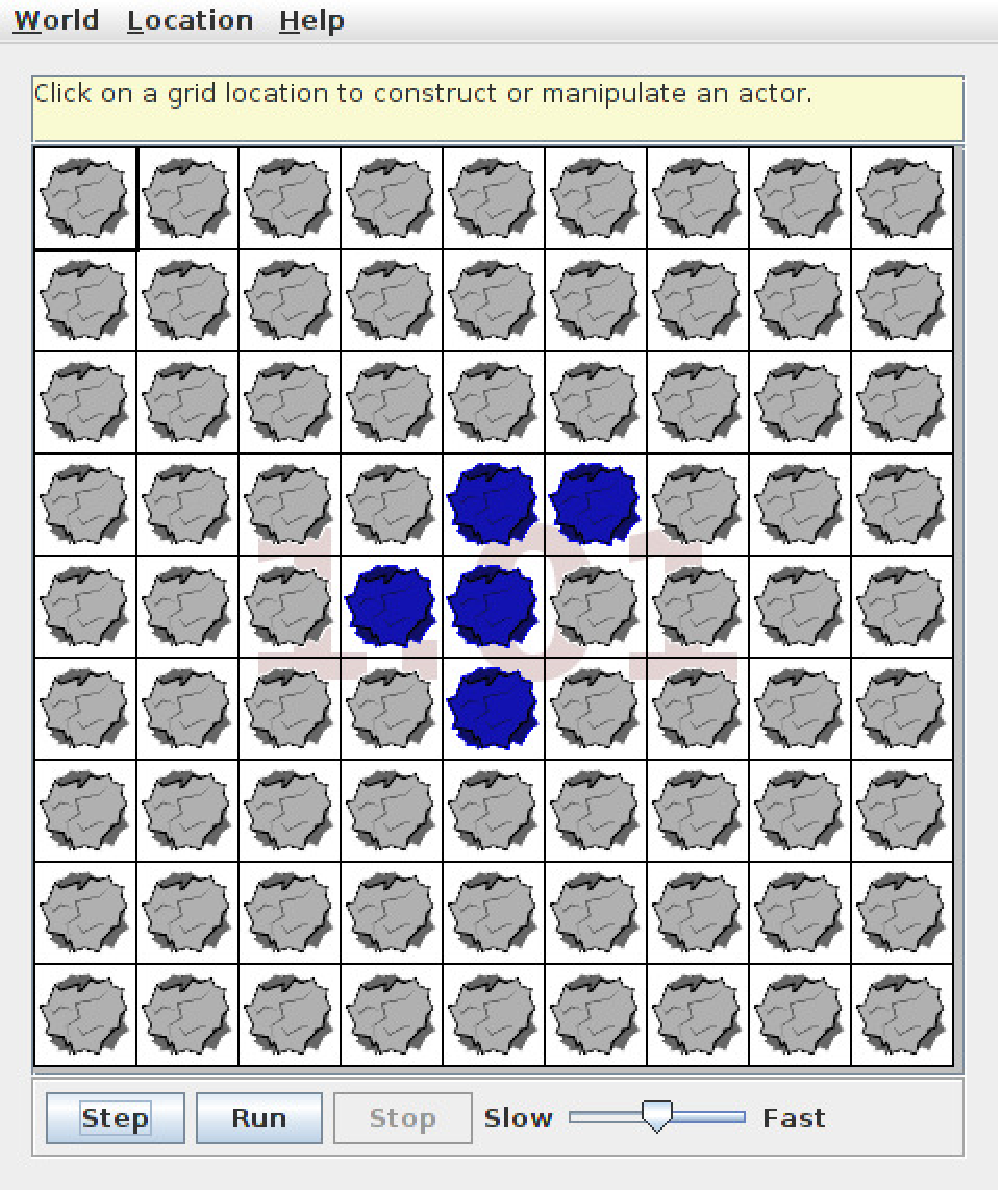
\includegraphics[height=2in]{figs/LifeRunner.pdf}

If you run this configuration for more than a few steps, it reaches the
end of the Grid.  The boundaries of the Grid change the behavior of
the system; in order to see the full evolution of the r-pentomino,
the Grid has to be big enough.  You might have to experiment to find
the right size, and depending on the speed of your computer, it
might take a while.

The Game of Life web page describes other initial conditions that
yield interesting results (\url{http://www.conwaylife.com/}).  Choose
one you like and implement it.

There are also variations of the Game of Life based on different rules.
Try one out and see if you find anything interesting.


\section{Vocabulary}

\begin{description}

\item[object method:]  A method that is invoked on an object,
and that operates on that object.
%, which is referred to by the keyword {\tt this} in Java
% or ``the current object'' in English.
Object methods do not have the keyword {\tt static}.

\item[class method:]  A method with the keyword {\tt static}.
Class methods are not invoked on objects and they do not have
a current object.

\item[current object:]  The object on which an object method
is invoked.  Inside the method,
the current object is referred to by {\tt this}.

%\item[{\tt this}:]  The keyword that refers to the current object.

\item[implicit:]  Anything that is left unsaid or implied.  Within
an object method, you can refer to the instance variables
implicitly (i.e., without naming the object).

\item[explicit:]  Anything that is spelled out completely.  Within
a class method, all references to the instance variables have to
be explicit.

\index{object method}
\index{class method}
\index{current object}
\index{this}
\index{implicit}
\index{explicit}

\end{description}


\section{Exercises}


\begin{exercise}
Starting with a copy of {\tt BlueBug.java}, write a class definition
for a new kind of {\tt Bug} that finds and eats flowers.  You can
``eat'' a flower by invoking {\tt removeSelfFromGrid} on it.
\end{exercise}


\begin{exercise}
Now you know what you need to know to read Part 3 of the
GridWorld Student Manual and do the exercises.
\end{exercise}


\begin{exercise}
If you implemented the Game of Life, you are well prepared for
Part 4 of the GridWorld Student Manual.  Read it and do the exercises.
\end{exercise}


\begin{exercise}

Download \url{http://thinkapjava.com/code/CardSoln2.java} and
\url{http://thinkapjava.com/code/CardSoln3.java}.

{\tt CardSoln2.java} contains solutions to the exercises
in the previous chapter.  It uses only class methods (except the
constructors).

{\tt CardSoln3.java} contains the same program, but most of the
methods are object methods.  I left {\tt merge} unchanged because
I think it is more readable as a class method.

Transform {\tt merge} into an object method,
and change {\tt mergeSort} accordingly.  Which version of
{\tt merge} do you prefer?

\end{exercise}


\begin{exercise}

Transform the following class method into an object method.

\begin{code}
public static double abs(Complex c) {
    return Math.sqrt(c.real * c.real + c.imag * c.imag);
}
\end{code}
\end{exercise}


\begin{exercise}
Transform the following object method into a class method.

\begin{code}
public boolean equals(Complex b) {
    return(real == b.real && imag == b.imag);
}
\end{code}
\end{exercise}


\begin{exercise}

This exercise is a continuation of Exercise~\ref{ex.rational}.
The purpose is to practice the syntax of object methods and
get familiar with the relevant error messages.

\begin{enumerate}

\item Transform the methods in the {\tt Rational} class
from class methods to object methods, and make the necessary
changes in {\tt main}.

\item Make a few mistakes.  Try invoking class methods as if
they were object methods and vice-versa.  Try to get a sense for
what is legal and what is not, and for the error messages that
you get when you mess up.

\item Think about the pros and cons of
class and object methods.  Which is more concise (usually)?
Which is a more natural way to express computation (or, maybe
more fairly, what kind of computations can be expressed most
naturally using each style)?

\end{enumerate}
\end{exercise}


\begin{exercise}
The goal of this exercise is to write a program that generates random
poker hands and classifies them, so that we can estimate the
probability of the various poker hands.  If you don't play poker, you
can read about it here
\url{http://en.wikipedia.org/wiki/List_of_poker_hands}.

\begin{enumerate}

\item Start with \url{http://thinkapjava.com/code/CardSoln3.java}
and make sure you can compile and run it.

\item Write a definition for a class named {\tt PokerHand}
that extends {\tt Deck}.

\item Write a {\tt Deck} method named {\tt deal} that creates
a PokerHand, transfers cards from the deck to the hand, and returns
the hand.

\item In {\tt main} use {\tt shuffle} and
{\tt deal} to generate and print four {\tt PokerHands} with
five cards each.  Did you get anything good?

\item Write a {\tt PokerHand} method called {\tt hasFlush}
returns a boolean indicating whether the
hand contains a flush.

\item Write a method called {\tt hasThreeKind} that
indicates whether the hand contains
Three of a Kind.

\item Write a loop that generates a few thousand hands and
checks whether they contain a flush or three of a kind.
Estimate the probability of getting one of those hands.
Compare your results to the probabilities at
\url{http://en.wikipedia.org/wiki/List_of_poker_hands}.

\item Write methods that test for the other poker hands.  Some
are easier than others.  You might find it useful to write some
general-purpose helper methods that can be used for more than one
test.

\item In some poker games, players get seven cards each, and
they form a hand with the best five of the seven.  Modify your
program to generate seven-card hands and recompute the probabilities.

\end{enumerate}
\end{exercise}


\end{document}
